\subsubsection{Complejidad}

En el caso de PageRank, la complejidad del algoritmo esta dictada por el tamaño del grafo que representa la red, con lo cual vamos a estudiar el tiempo de ejecucion en funcion de dicho factor.

Para generar las instancias tomamos igual cantidad de nodos y de ejes, la primera tomando valor 30, cada instancia sucesiva aumentamos la cantidad de nodos en 15, hasta llegar a las 150 iteraciones. En la matriz el tamaño esta dado en funcion de la cantidad de nodos, mientras que los ejes son utlizados en el paso inicial para determinar las probablidades iniciales, con lo cual la cantidad de ejes no tiene la misma importancia que la cantidad de nodos al calcular el metodo de la potencia.

El siguiente grafico muestra los tiempos de convergencia segun el tamaño, para suavizar el ruido se tomaron 5 muestras por cada instacia y tomamos el promedio.

\begin{figure}[H]
\centering
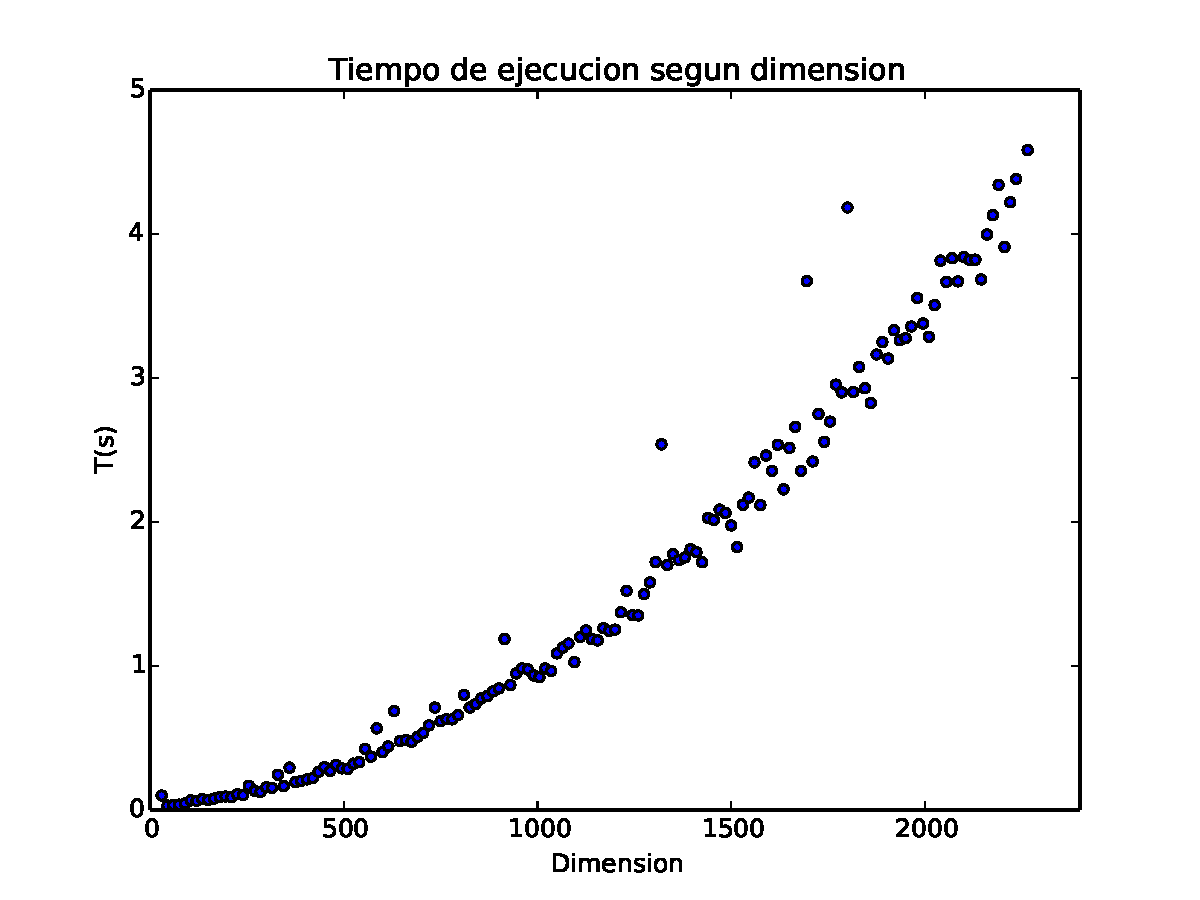
\includegraphics[scale=0.7]{images/complejidad.pdf}
\caption{Tiempos de ejecución según cantidad de webs.}
\label{timePageRank}
\end{figure}

Como podemos apreciar, el tiempo aumento de manera no lineal con respecto al tamaño de la entrada, lo cual es acorde al metodo de la potencia. Sin embargo, consideramos que es importante destacar que no hubo picos en el aumento (salvo casos aislados), es decir que el aumento fue gradual.